\documentclass[12pt]{article}

% ---------- Packages ----------
\usepackage[a4paper,margin=1in]{geometry}
\usepackage{mathptmx}              % Times New Roman look
\usepackage{setspace}              % Double spacing
\usepackage{microtype}
\usepackage{booktabs}
\usepackage{array}
\usepackage{amsmath,amssymb}
\usepackage{enumitem}
\usepackage{hyperref}
\usepackage{xurl}
\urlstyle{same}
\usepackage[dvipsnames]{xcolor}
\usepackage{graphicx}
\usepackage{float}
\usepackage{caption}
\usepackage{fancyhdr}
\usepackage{cite}                  % IEEE-style numeric citations
\usepackage{makecell}
\usepackage{IEEEtrantools}

% ---------- Spacing ----------
\doublespacing
\setlength{\parindent}{0.5in}
\setlength{\parskip}{0pt}

% ---------- Header / Footer ----------
\pagestyle{fancy}
\fancyhf{}
\lhead{
\includegraphics[height=24pt]{up-header.png}}
\rhead{\thepage}
\renewcommand{\headrulewidth}{0.4pt}
\setlength{\headheight}{40pt}

% ---------- Hyperlink setup ----------
\hypersetup{colorlinks=true,linkcolor=black,citecolor=black,urlcolor=black}
\Urlmuskip=0mu plus 1mu

\begin{document}

% Disable IEEEtran repeated-author dash shorthand in bibliography.
\bstctlcite{rfm_bstctl}

% ---------- Header Block ----------
\noindent Zildjian E. California\\
CMSC 125\\
\today

% ---------- Centered Title ----------
\begin{center}
Comparative CPU Scheduling: FCFS, SJF, RR, and Priority
\end{center}

% ---------- Required screenshot pages ----------
\begin{figure}[H]
  \centering
  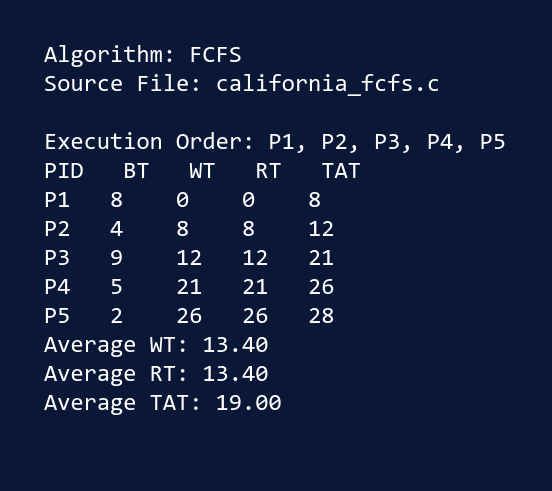
\includegraphics[width=\textwidth,height=0.78\textheight,keepaspectratio]{../artifacts/screenshots/01_fcfs.png}
  \caption{FCFS run output (\texttt{california\_fcfs.c}).}
\end{figure}
\clearpage

\begin{figure}[H]
  \centering
  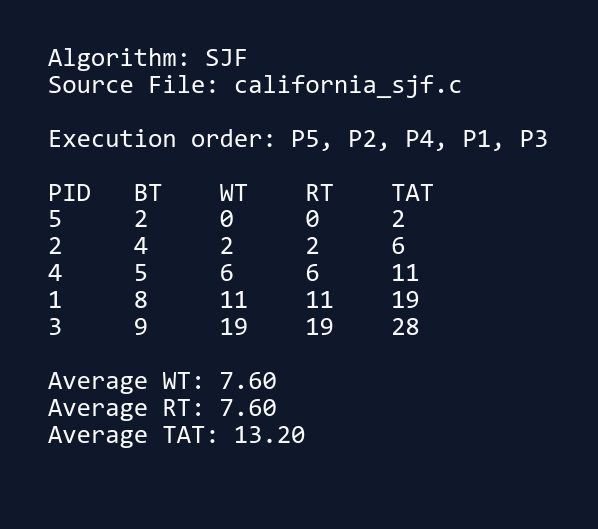
\includegraphics[width=\textwidth,height=0.78\textheight,keepaspectratio]{../artifacts/screenshots/02_sjf.png}
  \caption{SJF run output (\texttt{california\_sjf.c}).}
\end{figure}
\clearpage

\begin{figure}[H]
  \centering
  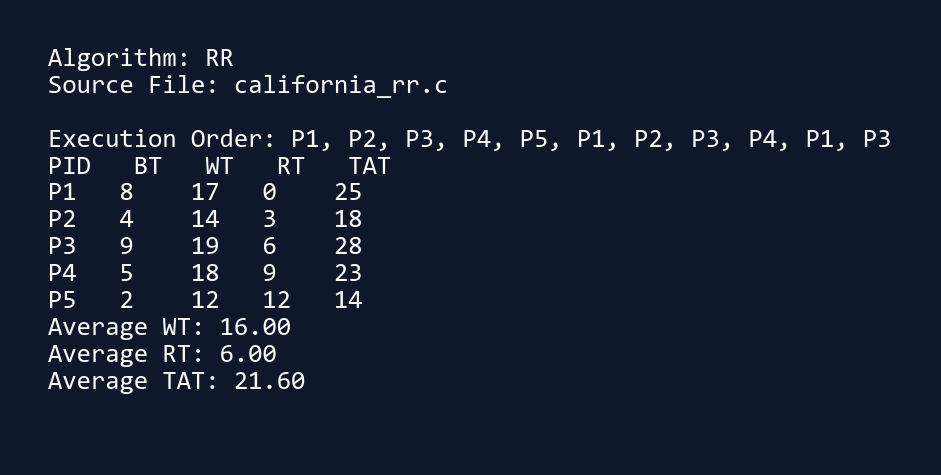
\includegraphics[width=\textwidth,height=0.78\textheight,keepaspectratio]{../artifacts/screenshots/03_rr.png}
  \caption{Round Robin run output (\texttt{california\_rr.c}, quantum = 3).}
\end{figure}
\clearpage

\begin{figure}[H]
  \centering
  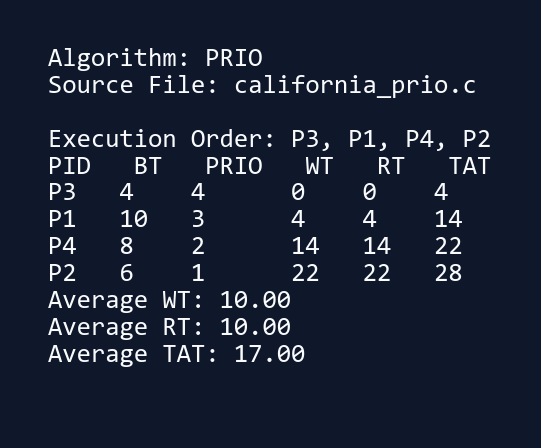
\includegraphics[width=\textwidth,height=0.78\textheight,keepaspectratio]{../artifacts/screenshots/04_prio.png}
  \caption{Priority (non-preemptive) run output (\texttt{california\_prio.c}).}
\end{figure}
\clearpage

% ---------- Comparative write-up ----------
\section*{Comparative Scheduling Write-up (FCFS vs SJF vs RR)}

\noindent This comparison is intentionally scoped to \textbf{FCFS, SJF, and RR only} (Priority excluded for \texttt{US-F2}). The implementation approach and algorithm definitions align with standard scheduling references \cite{studytonight_cpu,studytonight_fcfs,studytonight_sjf,studytonight_rr,studytonight_priority}.

\begin{singlespace}
\begin{table}[H]
  \centering
  \begin{tabular}{@{}lccc@{}}
    \toprule
    \textbf{Algorithm} & \textbf{AWT} & \textbf{ART} & \textbf{ATT} \\
    \midrule
    FCFS     & 13.40 & 13.40 & 19.00 \\
    SJF      & 7.60  & 7.60  & 13.20 \\
    RR (q=3) & 16.00 & 6.00  & 21.60 \\
    \bottomrule
  \end{tabular}
\end{table}
\end{singlespace}

\noindent\textbf{Average waiting time (AWT).} SJF is best (7.60) because shortest-first ordering minimizes cumulative waiting across the queue. RR is highest (16.00) because time slicing rotates work and reintroduces waiting between slices. FCFS lands between (13.40) because it preserves fixed arrival order and does not reorder by burst length.

\noindent\textbf{Average response time (ART).} RR is best (6.00) because round-robin dispatch caps time-to-first-slice at $(n-1)\cdot q = 12$ for this dataset, so every process gets CPU attention early. FCFS (13.40) and SJF (7.60) are non-preemptive and arrival is 0, so ART tracks each process's initial wait before first dispatch.

\noindent\textbf{Average turnaround time (ATT).} SJF is best (13.20) because early completion of short jobs reduces total completion-time accumulation. RR is highest (21.60) due to repeated queue cycling before completion. FCFS lands between (19.00) from fixed arrival order, no preemption cost, but no burst-aware ordering.

\newpage
\bibliographystyle{IEEEtran}
\bibliography{references}

\end{document}
